\chapter{Implementation}\label{sec:implementation}
\thispagestyle{fancy}

This chapter will describe implementation specific matters. However, it's not the purpose of this chapter to give a total understanding of all the implementation specific details. To get a in depth understanding the source code should be consulted. 

\section{Programming language and code}\label{sec:programming_language_and_code}
The \emph{Java} programming language were chosen as the platform for the solution. In addition there are \emph{HTML}, \emph{JavaScript} and \emph{CSS} code in the frontend. 

\section{Structure of solution}\label{sec:structure_of_solution}
There are five six level packages in the Solbrille source tree. These packages represent separate pieces of functionality and their roles may be summarized as following.

\begin{itemize}
	\item \texttt{com.ntnu.solbrille.buffering}: Used to do buffered IO and thread safe sharing of IO resources (Section~\ref{sec:buffered_io}).
	\item \texttt{com.ntnu.solbrille.feeder}: Used in the document preprocessing stage. This package contains two sub-packages: \texttt{outputs} for content targets, and \texttt{processors} for content processors (Section~\ref{sub:implemented_feeding_processors}).
	\item \texttt{com.ntnu.solbrille.index}: Contains the utilities for creating index structures, and three specific index implementations \texttt{content}, \texttt{document} and \texttt{occurence} (Section~\ref{sub:statistics_index_structure}-\ref{sub:occurrence_index_structure}). 
	\item \texttt{com.ntnu.solbrille.query}: The query processing pipeline, contains sub packages for preprocessing, matching, scoring and filtering. 
	\item \texttt{com.ntnu.solbrille.utils}: Utilities used in various parts of the solution. Contains a sub package for some special \emph{iterators} used during indexing and querying. 
	\item \texttt{com.ntnu.solbrille.frontend}: The web frontend for the search engine.
\end{itemize}

The relationships between these packages is summarized in Figure~\ref{fig:high_level_packages}. 

\begin{figure}[ht]
	\centering
%	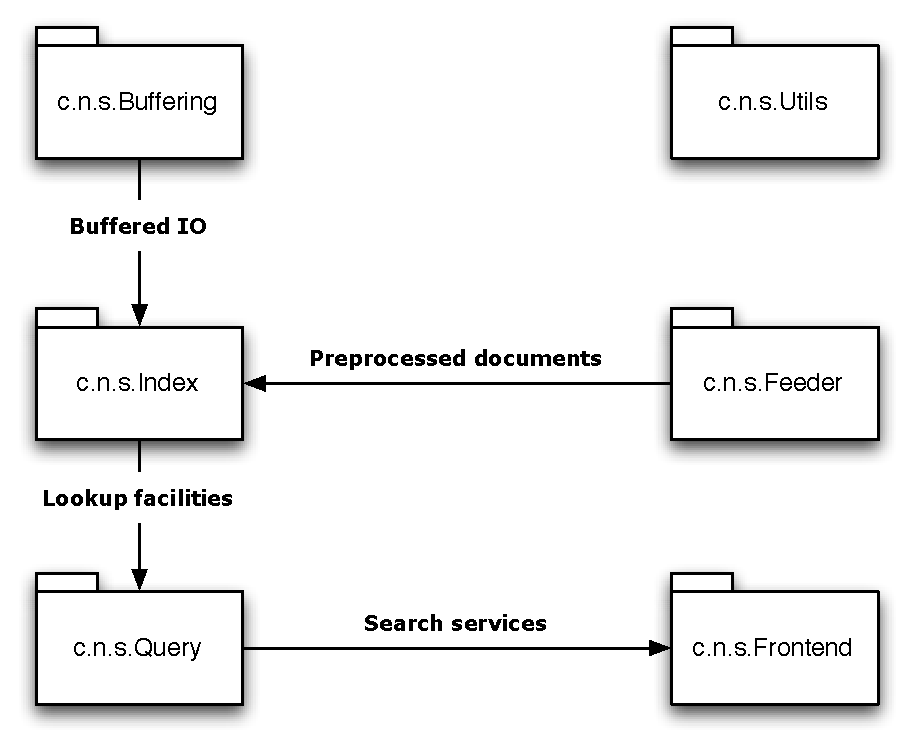
\includegraphics[width=0.6\textwidth]{include/packages.pdf}
	\caption{High level packages.}\label{fig:high_level_packages}
\end{figure}

\section{Index building and update algorithm}
The algorithm used for incrementally building and the occurrence index is as mentioned in Section~\ref{sub:index_building} a two phase algorithm. Initially one index update is built in memory, then when the index is flushed this update is merged with the existing index. 

The way this is managed to assure concurrent searches and index updating is that the system uses  two inverted files. One inverted file which is searched, and another one which is updated. To make the index consistent the concept of a \emph{Index phase} is introduced. A index phase is the identifier of the current searchable index. Each entry in the dictionary contains a double set of inverted list pointers, the current active set of pointers are determined by the parity of the current index phase. While merging the old inverted list and the new index update the inactive pointer of each dictionary entry is updated. When the update completes; the index phase is incremented and the active set of inverted list pointers are swapped (due to parity). 

\section{External libraries}\label{sec:external_libraries}
To ease the implementation some external libraries have been used. These libraries have been run past the course staff for verification.

\begin{itemize}
	\item \textbf{Snowball stemmer:} For stemming in the document and query preprocessing stage.
	\item \textbf{Carrot2 suffix tree:} For suffix tree clustering in the extended system. 
	\item \textbf{htmlparser.org:} To strip away \emph{HTML}-formatting from documents, to extract links for static link analysis etc.
	\item \textbf{Jetty:} A compact web-server to produce the frontend user interface. 	 
\end{itemize}